% Rascunho do short paper "khipu". Compilar neste diretório:  tectonic main.tex  (ou pdflatex + bibtex).
% Todo número de resultado vem de tables/numbers.tex e das tabelas, geradas por
% scripts/aggregate.py a partir de runs/khipu: NUNCA digite um resultado à mão.
% \todo{...} marca o que precisa ser conferido numa fonte antes de valer.
\documentclass[11pt]{article}
\usepackage[margin=1in]{geometry}
\usepackage[T1]{fontenc}
\usepackage{amsmath,amssymb}
\usepackage{booktabs}
\usepackage{graphicx}
\usepackage[dvipsnames]{xcolor}
\usepackage[colorlinks=true,allcolors=blue]{hyperref}

% gerado por scripts/aggregate.py: não editar à mão
\newcommand{\resKA}{1024}
\newcommand{\resKB}{8192}
\newcommand{\resMseSteKA}{3.63}
\newcommand{\resMseSdSteKA}{0.05}
\newcommand{\resPsnrSteKA}{24.40}
\newcommand{\resPsnrSdSteKA}{0.05}
\newcommand{\resUsedSteKA}{28.6}
\newcommand{\resUsedSdSteKA}{2.2}
\newcommand{\resPerpSteKA}{245.7}
\newcommand{\resPerpSdSteKA}{15.8}
\newcommand{\resFailedSteKA}{0/3}
\newcommand{\resMseSteEmaKA}{3.71}
\newcommand{\resMseSdSteEmaKA}{0.08}
\newcommand{\resPsnrSteEmaKA}{24.30}
\newcommand{\resPsnrSdSteEmaKA}{0.09}
\newcommand{\resUsedSteEmaKA}{24.4}
\newcommand{\resUsedSdSteEmaKA}{3.6}
\newcommand{\resPerpSteEmaKA}{202.6}
\newcommand{\resPerpSdSteEmaKA}{25.8}
\newcommand{\resFailedSteEmaKA}{0/3}
\newcommand{\resRatioMseSteEmaKAOverSte}{1.02}
\newcommand{\resRatioPerpSteEmaKAOverSte}{0.82}
\newcommand{\resRatioUsedSteEmaKAOverSte}{0.85}
\newcommand{\resMseGateNormKA}{6.31}
\newcommand{\resMseSdGateNormKA}{0.50}
\newcommand{\resPsnrGateNormKA}{22.01}
\newcommand{\resPsnrSdGateNormKA}{0.34}
\newcommand{\resUsedGateNormKA}{51.1}
\newcommand{\resUsedSdGateNormKA}{13.6}
\newcommand{\resPerpGateNormKA}{111.2}
\newcommand{\resPerpSdGateNormKA}{69.8}
\newcommand{\resFailedGateNormKA}{0/3}
\newcommand{\resRatioMseGateNormKAOverSte}{1.74}
\newcommand{\resRatioPerpGateNormKAOverSte}{0.45}
\newcommand{\resRatioUsedGateNormKAOverSte}{1.79}
\newcommand{\resMseGateCbKA}{4.35}
\newcommand{\resMseSdGateCbKA}{0.01}
\newcommand{\resPsnrGateCbKA}{23.61}
\newcommand{\resPsnrSdGateCbKA}{0.01}
\newcommand{\resUsedGateCbKA}{65.8}
\newcommand{\resUsedSdGateCbKA}{3.0}
\newcommand{\resPerpGateCbKA}{258.6}
\newcommand{\resPerpSdGateCbKA}{28.7}
\newcommand{\resFailedGateCbKA}{0/3}
\newcommand{\resRatioMseGateCbKAOverSte}{1.20}
\newcommand{\resRatioPerpGateCbKAOverSte}{1.05}
\newcommand{\resRatioUsedGateCbKAOverSte}{2.30}
\newcommand{\resMseDenseStKA}{3.34}
\newcommand{\resMseSdDenseStKA}{0.16}
\newcommand{\resPsnrDenseStKA}{24.76}
\newcommand{\resPsnrSdDenseStKA}{0.21}
\newcommand{\resUsedDenseStKA}{95.7}
\newcommand{\resUsedSdDenseStKA}{3.3}
\newcommand{\resPerpDenseStKA}{523.9}
\newcommand{\resPerpSdDenseStKA}{99.8}
\newcommand{\resFailedDenseStKA}{0/3}
\newcommand{\resRatioMseDenseStKAOverSte}{0.92}
\newcommand{\resRatioPerpDenseStKAOverSte}{2.13}
\newcommand{\resRatioUsedDenseStKAOverSte}{3.35}
\newcommand{\resMseSteKB}{4.10}
\newcommand{\resMseSdSteKB}{0.29}
\newcommand{\resPsnrSteKB}{23.88}
\newcommand{\resPsnrSdSteKB}{0.32}
\newcommand{\resUsedSteKB}{1.9}
\newcommand{\resUsedSdSteKB}{0.8}
\newcommand{\resPerpSteKB}{132.9}
\newcommand{\resPerpSdSteKB}{55.9}
\newcommand{\resFailedSteKB}{0/3}
\newcommand{\resMseGateCbKB}{2.86}
\newcommand{\resMseSdGateCbKB}{0.07}
\newcommand{\resPsnrGateCbKB}{25.44}
\newcommand{\resPsnrSdGateCbKB}{0.11}
\newcommand{\resUsedGateCbKB}{64.6}
\newcommand{\resUsedSdGateCbKB}{4.6}
\newcommand{\resPerpGateCbKB}{2303.7}
\newcommand{\resPerpSdGateCbKB}{138.9}
\newcommand{\resFailedGateCbKB}{0/3}
\newcommand{\resRatioMseGateCbKBOverSte}{0.70}
\newcommand{\resRatioPerpGateCbKBOverSte}{17.34}
\newcommand{\resRatioUsedGateCbKBOverSte}{33.99}
\newcommand{\resMseDenseStKB}{22.58}
\newcommand{\resMseSdDenseStKB}{34.00}
\newcommand{\resPsnrDenseStKB}{20.90}
\newcommand{\resPsnrSdDenseStKB}{7.64}
\newcommand{\resUsedDenseStKB}{37.1}
\newcommand{\resUsedSdDenseStKB}{28.5}
\newcommand{\resPerpDenseStKB}{1048.9}
\newcommand{\resPerpSdDenseStKB}{393.0}
\newcommand{\resFailedDenseStKB}{1/3}
\newcommand{\resRatioMseDenseStKBOverSte}{5.50}
\newcommand{\resRatioPerpDenseStKBOverSte}{7.89}
\newcommand{\resRatioUsedDenseStKBOverSte}{19.51}
\newcommand{\resBaselineMse}{61.8}
\newcommand{\resFailFraction}{0.95}
\newcommand{\resNSeeds}{3}
\newcommand{\resPilotRuns}{9}
\newcommand{\resPilotFailed}{3}


\newcommand{\todo}[1]{{\color{red}[TODO: #1]}}
\newcommand{\sg}{\operatorname{sg}}
\newcommand{\ebar}{\bar{e}}
\newcommand{\est}[1]{\texttt{#1}}

\title{Gate-Value Gradients for Vector Quantization:\\
       the VQ Layer as a Degenerate Mixture of Experts}
\author{\todo{authors}}
\date{Preliminary draft}

\begin{document}
\maketitle

\begin{abstract}
A vector-quantized VAE makes one discrete decision per token, the nearest codeword, and trains the
encoder through it with the straight-through estimator (STE). A sparse mixture-of-experts (MoE)
layer makes the same kind of decision with a router, which is trained with a different estimator,
the gradient of the gate value. We observe that a VQ layer is a degenerate MoE (codewords are
constant experts, the nearest neighbour is a top-1 router) and compare STE with three gate-value
estimators, on a 2-D toy and on CIFAR-10 with two codebook sizes. In this preliminary study
(\resNSeeds{} seeds per cell) a dense gate estimator reaches the lowest reconstruction error
at $K=\resKA$, the normalised gate-value estimator is worse than STE there, and a gate estimator that
keeps STE on the encoder uses far more of the codebook; but one dense-gate run at $K=\resKB$
did not learn. We report all of it, including what contradicts our expectations.
\end{abstract}

\section{Introduction}
Vector quantization (VQ) in a VQ-VAE~\cite{vandenoord2017vqvae} and expert routing in a sparse
mixture of experts~\cite{shazeer2017moe,fedus2021switch} both turn a continuous quantity into a
discrete choice. The two layers train through that choice differently. The VQ-VAE uses the
straight-through estimator~\cite{bengio2013ste}, which copies the gradient from the quantized
vector to the encoder output. The MoE router is trained through the gate value, which multiplies
the expert output and carries a gradient to the router
\todo{confirm that Switch/Shazeer train the router through the gate value as described}.

In MoE layers an estimator that sends a gradient to experts that were not selected requires
evaluating them, which is expensive \todo{confirm in the MoE literature that this cost is the
reason straight-through-style estimators were avoided for routing}. In a VQ layer this objection
does not apply: the ``experts'' are constant codewords, so all $K$ expert outputs are already
available.

We therefore ask whether the router-style gradient is a better estimator for the VQ layer. We
state two hypotheses before looking at the results:
\textbf{H1}, the normalised gate-value estimator (\est{gate\_norm}) yields a worse encoder, and
hence a worse reconstruction, than STE; \textbf{H2}, a gate-value estimator that keeps STE on the
encoder and applies the gate value only to the codebook (\est{gate\_cb}) improves codebook usage.
Our contributions are modest: (i) the VQ$\to$MoE correspondence written out (Sec.~2); (ii) three
gate-value estimators with closed-form gradients, checked against automatic differentiation
(Sec.~3); (iii) a small empirical comparison with STE (Sec.~4).

\emph{Related directions} (cited by title only; \todo{every statement about how these relate to
our work must be checked against the papers; we make no novelty claim}): gradient estimation for
sparse routing~\cite{liu2023sparsemixer,liu2024grin,panda2025defaultmoe}, estimators for
vector-quantized networks~\cite{huh2023straightening,fifty2024rotation}, connections between
discrete representations and MoE~\cite{do2024vqmoe,zhong2026rqmoe}, and routed language
models~\cite{clark2022unified}.

\section{VQ as a degenerate mixture of experts}
Let $z\in\mathbb{R}^d$ be an encoder output (one per token) and $e_1,\dots,e_K$ the codewords.
With $d_j=\lVert z-e_j\rVert^2$,
\begin{equation}
  k^\star=\arg\min_j d_j,\qquad p_j=\operatorname{softmax}_j\!\bigl(-d_j/\tau\bigr),\qquad
  \bar e=\sum_j p_j e_j .
\end{equation}
A top-1 MoE layer computes $y=g_{k^\star}(x)\,f_{k^\star}(x)$ with a router that selects
$k^\star$. Taking $f_j(x)=e_j$ (constant experts) and a router with logits $-\lVert z-e_j\rVert^2$
gives the VQ layer, whose forward output is $z_q=e_{k^\star}$:
\begin{center}
\small
\begin{tabular}{ll}
\toprule
MoE & VQ layer \\
\midrule
token / input $x$ & encoder output $z$ \\
expert $f_j$ & constant codeword $e_j$ \\
router logits & $-\lVert z-e_j\rVert^2$ \\
top-1 selection & nearest neighbour $k^\star$ \\
router probabilities $p$ & $\operatorname{softmax}(-d/\tau)$ \\
output $g_{k^\star}f_{k^\star}$ & $e_{k^\star}$ (gate fixed to 1 in the forward pass) \\
\bottomrule
\end{tabular}
\end{center}
The only difference in the forward pass is that VQ does not multiply by the gate value. The
estimators below restore the gate value \emph{in the backward pass only}: they divide the gate
by its own stop-gradient, $p_{k^\star}/\sg(p_{k^\star})$, which equals $1$ in the forward pass.
\todo{check prior work on this correspondence~\cite{do2024vqmoe,zhong2026rqmoe} before claiming it
as an observation of ours}

\section{Estimators}
In every case the forward output is exactly $e_{k^\star}$; they differ in the gradient. Let
$g=\partial L/\partial z_q$, $\sg$ the stop-gradient, and add the commitment loss
$\beta\lVert z-\sg(e_{k^\star})\rVert^2$ ($\beta=0.25$) to all of them.
\begin{itemize}\setlength\itemsep{2pt}
\item \est{ste}: $z_q=z+\sg(e_{k^\star}-z)$, with the codebook loss $\lVert \sg(z)-e_{k^\star}\rVert^2$.
  $\partial L/\partial z=g$. \est{ste\_ema} is the same with the codebook updated by an
  exponential moving average (decay $0.99$) and no codebook loss.
\item \est{gate\_norm}: $z_q=\dfrac{p_{k^\star}}{\sg(p_{k^\star})}\,e_{k^\star}$. Since
  $\nabla_z\log p_{k^\star}=\tfrac{2}{\tau}(e_{k^\star}-\bar e)$,
  \begin{equation}
    \frac{\partial L}{\partial z}=\frac{2}{\tau}\,(g\!\cdot\! e_{k^\star})\,(e_{k^\star}-\bar e).
  \end{equation}
  It vanishes when the assignment becomes one-hot ($\bar e\to e_{k^\star}$).
\item \est{gate\_cb}: $z_q=z-\sg(z)+\dfrac{\hat p_{k^\star}}{\sg(\hat p_{k^\star})}\,e_{k^\star}$,
  with $\hat p$ computed from $\sg(z)$. The encoder receives exactly $g$ (STE), and the gate value
  acts only on the codebook. An optional codebook loss exists and is off here.
\item \est{dense\_st}: $z_q=\bar e+\sg(e_{k^\star}-\bar e)$. The forward output is $e_{k^\star}$ and
  the backward pass goes through the full mixture $\bar e$:
  \begin{equation}
    \frac{\partial L}{\partial z}=\frac{2}{\tau}\sum_j p_j\,(g\!\cdot\! e_j)\,(e_j-\bar e).
  \end{equation}
\end{itemize}
\est{gate\_norm}, \est{gate\_cb} and \est{dense\_st} use no codebook loss by default. We checked
the three closed-form gradients against automatic differentiation in float64 (tolerance $10^{-6}$)
in the unit tests of the code. The temperature is $\tau\times\operatorname{median}_i
\lVert z_i-e_{k^\star}\rVert^2$, with the median estimated on the first batch and then frozen.

\begin{figure}[t]
\centering
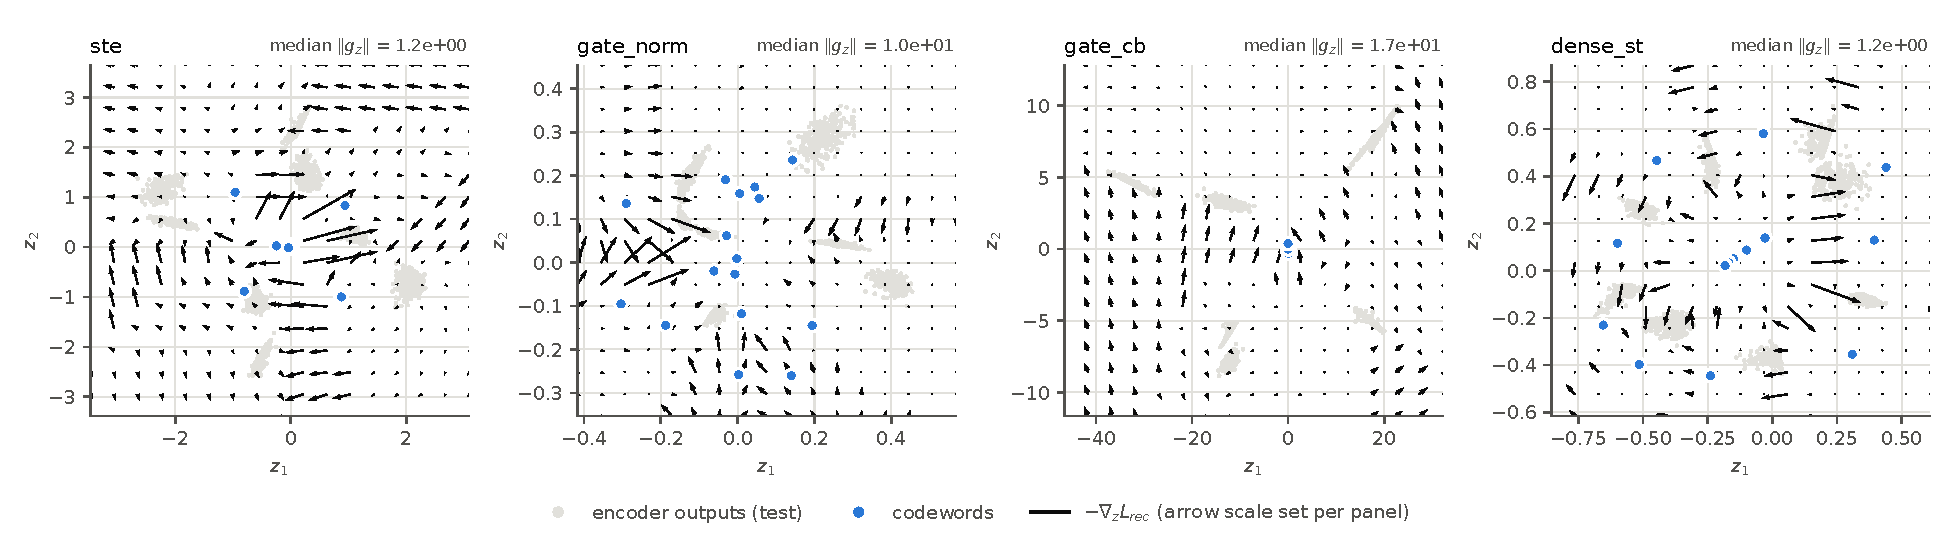
\includegraphics[width=\textwidth]{figures/fig_toy_field_s0.pdf}\\[2pt]
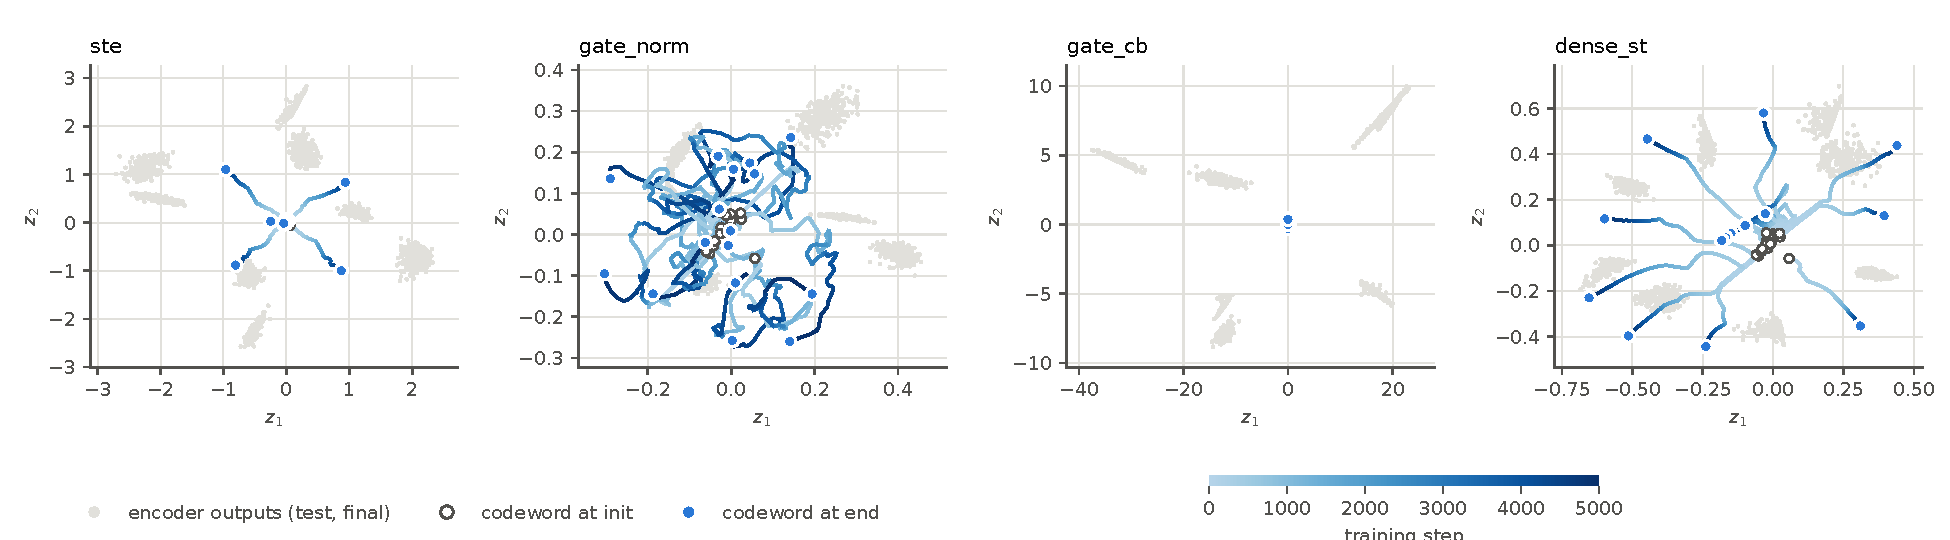
\includegraphics[width=\textwidth]{figures/fig_toy_traj_s0.pdf}
\caption{Toy 2-D problem (8 Gaussians on a ring, MLP encoder and decoder with $d=2$, $K=16$
codewords), seed 0 of 3. \textbf{Top:} $-\nabla_z L_{rec}$ on a grid of latent points; the target
of each point is the test sample whose latent is closest to it, and the arrow scale is set per
panel (the median gradient norm is printed above each panel). \textbf{Bottom:} path of each
codeword during training. This only illustrates the mechanism; it is not evidence for H1 or H2.}
\label{fig:toy}
\end{figure}

Figure~\ref{fig:toy} shows what the estimators do in the plane. With \est{gate\_cb} the encoder
outputs spread over a much wider range than with the other estimators while the codewords stay
close to the origin; the \est{gate\_norm} codewords follow tangled paths, and the \est{dense\_st}
codewords move smoothly towards the data. These are observations on one seed of a toy problem.

\section{Preliminary results}
\textbf{Setup.} CIFAR-10, a small convolutional VQ-VAE (two $4\times4$ stride-2 convolutions, two
residual blocks, 128 channels, $d=64$, so $8\times8$ tokens per image), Adam with learning rate
$3\cdot10^{-4}$, batch size 128, 20k steps, the same uniform codebook initialisation for every
estimator and no dead-code reinitialisation. We report test reconstruction metrics at the last step
for $K\in\{\resKA,\resKB\}$ and seeds 0--2; at $K=\resKB$ only \est{ste}, \est{gate\_cb} and
\est{dense\_st} were run. Perplexity is $\exp$ of the entropy of the codeword usage on the test
set. The value of $\tau$ was chosen per estimator in a small pilot (Sec.~5).

\begin{table}[t]
\centering
\small
\resizebox{\textwidth}{!}{\begin{tabular}{rllrccccr}
\toprule
$K$ & Estimator & $\tau$ & $n$ & MSE ($\times 10^{-3}$) & PSNR (dB) & Codes used (\%) & Perplexity & Failed$^\dagger$ \\
\midrule
1024 & \texttt{ste} & -- & 3 & 3.63 $\pm$ 0.05 & 24.40 $\pm$ 0.05 & 28.6 $\pm$ 2.2 & 245.7 $\pm$ 15.8 & 0/3 \\
 & \texttt{ste\_ema} & -- & 3 & 3.71 $\pm$ 0.08 & 24.30 $\pm$ 0.09 & 24.4 $\pm$ 3.6 & 202.6 $\pm$ 25.8 & 0/3 \\
 & \texttt{gate\_norm} & 0.1 & 3 & 13.51 $\pm$ 3.24 & 18.77 $\pm$ 1.00 & 12.9 $\pm$ 3.6 & 17.0 $\pm$ 5.4 & 0/3 \\
 & \texttt{gate\_cb} & 1 & 3 & 4.35 $\pm$ 0.01 & 23.61 $\pm$ 0.01 & 65.8 $\pm$ 3.0 & 258.6 $\pm$ 28.7 & 0/3 \\
 & \texttt{dense\_st} & 0.01 & 3 & 3.37 $\pm$ 0.01 & 24.72 $\pm$ 0.01 & 75.2 $\pm$ 3.0 & 499.1 $\pm$ 15.2 & 0/3 \\
\midrule
8192 & \texttt{ste} & -- & 3 & 4.10 $\pm$ 0.29 & 23.88 $\pm$ 0.32 & 1.9 $\pm$ 0.8 & 132.9 $\pm$ 55.9 & 0/3 \\
 & \texttt{gate\_cb} & 1 & 3 & 2.86 $\pm$ 0.07 & 25.44 $\pm$ 0.11 & 64.6 $\pm$ 4.6 & 2303.7 $\pm$ 138.9 & 0/3 \\
 & \texttt{dense\_st} & 0.03 & 3 & 2.66 $\pm$ 0.05 & 25.76 $\pm$ 0.08 & 39.8 $\pm$ 4.2 & 1900.4 $\pm$ 190.9 & 0/3 \\
\bottomrule
\end{tabular}
}
\caption{CIFAR-10 test metrics at step 20k, mean $\pm$ sample standard deviation over seeds.
$\tau$ is the multiple of the median $\lVert z-e_{k^\star}\rVert^2$ of the first batch, chosen per
estimator on the test set from a seed-0 pilot at $K=\resKA$ (\est{ste} and \est{ste\_ema} do not use
it). $^\dagger$Number of runs whose test MSE is at least $\resFailFraction$ times the MSE of
predicting the training mean image ($\resBaselineMse\times10^{-3}$); a post-hoc descriptive
criterion.}
\label{tab:main}
\end{table}

Table~\ref{tab:main} has the numbers. We run no significance tests; with \resNSeeds{} seeds the
standard deviations are only indicative.

\textbf{H1.} At $K=\resKA$, \est{gate\_norm} reaches an MSE of $\resMseGateNormKA\times10^{-3}$
against $\resMseSteKA\times10^{-3}$ for \est{ste} (ratio $\resRatioMseGateNormKAOverSte$), and its
spread across seeds is larger. This is consistent with H1. It is a whole-model measure: we did not
isolate the encoder (Sec.~5). \est{gate\_norm} uses more codewords than \est{ste}
($\resUsedGateNormKA\%$ against $\resUsedSteKA\%$) but its usage is less uniform
(perplexity $\resPerpGateNormKA$ against $\resPerpSteKA$).

\textbf{H2.} \est{gate\_cb} uses more of the codebook than \est{ste} at both sizes
($\resUsedGateCbKA\%$ against $\resUsedSteKA\%$ at $K=\resKA$, and $\resUsedGateCbKB\%$ against
$\resUsedSteKB\%$ at $K=\resKB$). The perplexity gain is large only at $K=\resKB$
($\resPerpGateCbKB$ against $\resPerpSteKB$), while at $K=\resKA$ it is similar
($\resPerpGateCbKA$ against $\resPerpSteKA$). Better usage does not give lower error at
$K=\resKA$ (MSE ratio $\resRatioMseGateCbKAOverSte$ to \est{ste}), but does at $K=\resKB$
($\resMseGateCbKB\times10^{-3}$ against $\resMseSteKB\times10^{-3}$, ratio
$\resRatioMseGateCbKBOverSte$). So H2 holds for codebook usage, and for reconstruction only at the
larger codebook.

\textbf{\est{dense\_st}.} At $K=\resKA$ it has the lowest mean MSE
($\resMseDenseStKA\times10^{-3}$) and the highest usage ($\resUsedDenseStKA\%$, perplexity
$\resPerpDenseStKA$). At $K=\resKB$ one of the three seeds (seed 0) did not learn: its test MSE
equals that of predicting the mean image, although its codebook was still in use. This is flagged
in the last column of Table~\ref{tab:main} and inflates the mean and the spread
($\resMseDenseStKB\pm\resMseSdDenseStKB\times10^{-3}$); the other two seeds are comparable to
\est{gate\_cb}. We did not investigate the cause. \est{ste\_ema} is close to \est{ste} at
$K=\resKA$. For \est{ste}, going from $K=\resKA$ to $K=\resKB$ did not reduce the error
($\resMseSteKA\times10^{-3}$ to $\resMseSteKB\times10^{-3}$) and left only $\resUsedSteKB\%$ of the
codewords in use.

\section{Limitations and next steps}
\begin{itemize}\setlength\itemsep{2pt}
\item \textbf{Selecting $\tau$ on the test set.} $\tau$ was chosen per estimator by the best final
  test MSE in a pilot of $\resPilotRuns$ runs (seed 0, $K=\resKA$), because no single $\tau$
  suits all estimators: $\resPilotFailed$ of the pilot runs did not learn (same criterion as
  in Table~\ref{tab:main}). There is
  no validation split, so the reported numbers are optimistic for the gate estimators. The
  seed-0 runs of the main grid are the same runs as in the pilot, the value chosen for
  \est{dense\_st} lies at the edge of the tested grid, and the same $\tau$ was reused at
  $K=\resKB$ without re-tuning (where one \est{dense\_st} seed did not learn).
\item \textbf{Few seeds, one dataset, one metric.} \resNSeeds{} seeds, CIFAR-10 only, and
  reconstruction metrics only, with a fixed 20k-step budget.
\item \textbf{The encoder is not isolated.} H1 is about the encoder, but we measured
  reconstruction of the whole model; a probe on frozen latents, or a fixed decoder, would separate
  the two.
\item \textbf{Post-hoc failure criterion.} The ``did not learn'' flag was defined after seeing the
  data, anchored on the mean-image MSE.
\end{itemize}
\textbf{Next steps} (to be decided): select $\tau$ on a held-out split of the training set; study
why \est{dense\_st} fails at $K=\resKB$ for one seed; re-estimate the median in $\tau$ during
training instead of freezing it on the first batch; evaluate the codebook-loss option of
\est{gate\_cb}; and test more datasets and codebook sizes.

\bibliographystyle{plain}
\bibliography{refs}
\end{document}
